\documentclass[a4paper,conference,10pt]{IEEEtran}
\usepackage[T1]{fontenc}
\usepackage{lmodern}
\usepackage{graphicx}
\usepackage{amsmath,amssymb}
\usepackage{booktabs}
\usepackage{cite}
\usepackage{url}
\usepackage{balance}
\hyphenation{Starobinsky PolyChord cosmo-logical}
\begin{document}
\title{Latency--Reliability Tradeoffs in Neural-Ensemble Surrogates for Cosmological Likelihood Evaluation}
\author{\IEEEauthorblockN{Marvin Francisco Jim\'enez Pe\~nafiel, Clara In\'es Rojas Cely}
\IEEEauthorblockA{School of Physical Sciences and Nanotechnology\\
Universidad de Investigaci\'on de Tecnolog\'ia Experimental Yachay (Yachay Tech)\\
Urcuqu\'i, Ecuador}}
\maketitle
\begin{abstract}
Our original PolyChord calculations for Starobinsky inflation required repeated Cobaya--CLASS likelihood evaluations. Here we ask a more deeply computational question: when can a neural ensemble approximate those evaluations, and what happens when its error is used as though it were an exact likelihood? We examine SR1, SR2, and a $\Lambda$CDM+$r$ reference using the same Planck 2018 and BICEP/Keck 2018 likelihood components. Five-network ensembles require 1.21--1.25\,ms per point, compared with 8.50--17.69\,s for direct evaluations on the same CPU node; the corresponding per-call ratios are $6.78\times10^3$--$1.46\times10^4$. Thirty-six independent replays reproduce stored exact $\chi^2$ values within $2.3\times10^{-13}$. Speed, however, is not the limiting issue. On 100 deliberately mixed external points per model, $R^2$ is 0.569--0.909, and the networks underestimate $\chi^2$ severely in some poorly represented regions. Reweighting the original chains with these predictions concentrates posterior weights onto a few such points. We therefore tested ensemble disagreement and distance to posterior-supported training samples as signals for exact fallback. Thresholds fixed using an earlier targeted experiment were applied, before CLASS evaluation, to 108 separately seeded proposals. Among 75 valid evaluations, all 13 underpredictions exceeding 50 $\chi^2$ units were flagged by each of the three tested gates, with different evaluation costs. These pointwise results motivate selective exact checks; they do not establish an accurate surrogate posterior or a measured speedup for a complete hybrid sampler.
\end{abstract}
\begin{IEEEkeywords}
Neural-network ensembles, scientific computing, uncertainty estimation, latency benchmarking, cosmological likelihoods, selective evaluation.
\end{IEEEkeywords}

\section{Introduction}
The PolyChord analysis underlying this work required repeated calls to Cobaya~\cite{torrado2021} and CLASS~\cite{blas2011} for each proposed cosmological parameter vector. Every call propagates primordial perturbations to CMB observables and evaluates the Planck 2018~\cite{planck2020} and BICEP/Keck 2018~\cite{bk2021} likelihood terms. This made our three original inference cases---two slow-roll implementations of Starobinsky inflation~\cite{starobinsky1980} and a $\Lambda$CDM+$r$ reference---a useful setting for measuring the practical cost of replacing direct evaluations with previously trained networks. PolyChord~\cite{handley2015} supplied the chains from which the emulator data were assembled.

There are already strong precedents for neural acceleration in cosmology. CosmoPower~\cite{mancini2022} predicts power spectra, while CONNECT~\cite{nygaard2023} emulates cosmological observables and has tested the recovery of posterior distributions. Our target is different: we return the total and individual likelihood contributions, expressed as $\chi^2$. This avoids running again the forward calculation for each trial point, but it also makes error in the learned function enter the posterior exponentially. A low prediction error averaged over familiar points may therefore hide a much larger problem in sparsely sampled regions. Ensemble disagreement is a useful warning signal~\cite{lakshminarayanan2017}, not by itself a calibrated error interval~\cite{guo2017}.

We first separate computational latency from prediction quality. We then examine the consequence of surrogate errors for the weights of existing posterior samples and test whether pre-specified rules can identify large errors at new parameter coordinates. The experiments concern likelihood calls and exact-fallback decisions; no surrogate-driven nested-sampling run is claimed.

\section{Likelihood Surrogates and Experimental Protocol}
\subsection{Physical inflationary configurations}
The Starobinsky $R+R^2$ model is equivalent, in the Einstein frame,
to a scalaron $\phi$ with the plateau potential
\begin{equation}
 V(\phi)=\frac{3}{4}M^2M_{\rm Pl}^2
 \left(1-e^{-\sqrt{2/3}\,\phi/M_{\rm Pl}}\right)^2.
 \label{eq:potential}
\end{equation}
Here $M_{\rm Pl}$ is the reduced Planck mass. The two numerical
slow-roll prescriptions in this study are \emph{not} distinct potentials:
they implement different approximations for the primordial observables
as functions of the e-fold number $N_*$, namely
\begin{align}
 n_s^{\rm SR1}&=1-\frac{2}{N_*}-\frac{9}{2N_*^2}, &
 r_{0.05}^{\rm SR1}&=\frac{12}{N_*^2}, \nonumber\\
 \alpha_s^{\rm SR1}&=0, & & \label{eq:sr1}\\[-1mm]
 n_s^{\rm SR2}&=1-\frac{2}{N_*}-\frac{3}{2N_*^2}, &
 r_{0.05}^{\rm SR2}&=\frac{12}{N_*^2}\left(1-\frac{2}{N_*}\right),\nonumber\\
 \alpha_s^{\rm SR2}&=-\frac{2}{N_*^2}-\frac{3}{N_*^3}. && \label{eq:sr2}
\end{align}
We use $50\leq N_*\leq60$ and pivot $k_*=0.05\,{\rm Mpc}^{-1}$. The flat $\Lambda$CDM+$r$ reference independently samples $n_s\in[0.94,0.99]$ and $r_{0.05}\in[0,0.08]$. The likelihood data remain identical across models; SR1--SR2 differences derive from the relations above.

\subsection{Forward evaluations and training data}
For parameter vector $\boldsymbol\theta$, the reference quantity is the total likelihood contribution expressed as
\begin{equation}
\chi^2(\boldsymbol\theta)=-2\log \mathcal{L}(\boldsymbol\theta)+C,
\label{eq:chi}
\end{equation}
where the additive convention $C$ is fixed by the corresponding likelihood implementation. We approximate the stored total $\chi^2$ and four constituent contributions (BICEP/Keck, Planck high-$\ell$ TTTEEE-lite, and Planck low-$\ell$ EE and TT). Comparisons use a \emph{matched} likelihood configuration; absolute $\chi^2$ values are not compared across incompatible likelihood implementations.

We reused evaluations from the definitive PolyChord chains, preparing a separate data set for each model rather than pooling different parameterizations. SR1 and SR2 have 14 inputs, with $N_*$ determining their primordial observables; the $\Lambda$CDM+$r$ data have 15, including independently sampled $n_s$ and $r$. The targets are the total and four component $\chi^2$ values. The training/validation/test partitions contain 5,931/1,271/1,272 (SR1), 5,886/1,261/1,262 (SR2), and 6,360/1,363/1,363 ($\Lambda$CDM+$r$) points. Scaling parameters were fitted only on each training partition. The present experiments reload the saved networks and inverse-transform their outputs; no additional training was performed.

\subsection{Five-member neural ensembles}
Each model uses $M=5$ independently stored multilayer perceptrons with hidden widths 128, 96, and 64, SiLU nonlinearities, batch normalization, and dropout 0.05 during training. For the total-$\chi^2$ prediction, the reported mean and empirical network dispersion are
\begin{align}
\widehat{\chi^2}(\boldsymbol\theta)&=\frac{1}{M}\sum_{m=1}^{M}\widehat{\chi^2}_m(\boldsymbol\theta),\label{eq:mean}\\[-1mm]
 s(\boldsymbol\theta)&=\operatorname{std}_{m=1,\ldots,M}\!\left[\widehat{\chi^2}_m(\boldsymbol\theta)\right].\label{eq:sigma}
\end{align}
We interpret $s$ as the spread of five fitted predictions, not a posterior standard deviation or a frequentist coverage guarantee. Reloading the checkpoints reproduced the previously stored neural outputs to within $6\times10^{-5}$ in $\chi^2$.

\subsection{Hardware, timing and reference verification}
We used the CEDIA node \texttt{compute-0-2} with identical recorded CPU affinity (logical CPUs 29 and 157) and one compute thread. Cobaya--CLASS ran in \texttt{inflacion}; the neural tests used CPU-only PyTorch. Neural timing includes scaling, five network passes, inverse scaling, and aggregation, but not loading checkpoints. Each batch size (1, 16, 64, 256, 1,024) was timed on 3,000 predictions over three repeats. The 12 exact calls per model followed a separate warm-up and exclude initialization. Different software environments and numbers of timed points limit comparability beyond per-call latency.

\subsection{External candidate selection and diagnostics}
Each external set contains 100 successfully evaluated candidates partitioned into four equal strata: \texttt{random}, \texttt{acquisition}, \texttt{low\_chi2}, and \texttt{uncertainty}. We report mean absolute error (MAE), root mean squared error (RMSE), $R^2$, Spearman rank correlation $\rho(s,|\Delta\chi^2|)$, and the empirical fractions satisfying $|\Delta\chi^2|\leq s$ and $|\Delta\chi^2|\leq2s$. These are descriptive coverages, \emph{not} nominal probabilistic intervals.

We deliberately included difficult candidates; pooling the four strata therefore exaggerates their prevalence relative to a genuinely random posterior draw.

\section{Results}
\subsection{Exact reproducibility and latency}
All 36 exact repeats (12/model) reproduce the corresponding stored $\chi^2$ values, with maximum absolute discrepancy $2.27\times10^{-13}$. Table~\ref{tab:perf} compares the median exact time with the single-point neural ensemble latency. The measured ratio is
\begin{equation}
S_{\mathrm{call}}=\frac{t_{\mathrm{exact,median}}}{t_{\mathrm{ensemble,batch=1}}}.\label{eq:speedup}
\end{equation}
The per-call ratios range from $6.78\times10^{3}$ for SR1 to $1.46\times10^{4}$ for SR2. Batched inference reaches approximately $1.48$--$1.50\times10^{5}$ predictions/s at batch size 1,024, reflecting throughput-oriented amortization rather than a second comparison to exact CLASS calls.

\begin{table}[t]
\caption{Matched-node per-call timing and external prediction errors. Exact: median of 12 distinct calls; ensemble: batch-size-one latency. Errors: 100 selected external points per model.}
\label{tab:perf}
\centering
\footnotesize
\setlength{\tabcolsep}{3.1pt}
\begin{tabular}{@{}lrrrrr@{}}
\toprule
Model & Exact (s) & NN (ms) & $S_{\rm call}$ & RMSE & $R^2$\\
\midrule
SR1 & 8.496 & 1.253 & 6,781$\times$ & 4.549 & 0.710 \\
SR2 & 17.685 & 1.212 & 14,593$\times$ & 6.964 & 0.569 \\
$\Lambda$CDM+$r$ & 17.659 & 1.218 & 14,499$\times$ & 2.946 & 0.909 \\
\bottomrule
\end{tabular}
\end{table}

\begin{figure}[t]
\centering
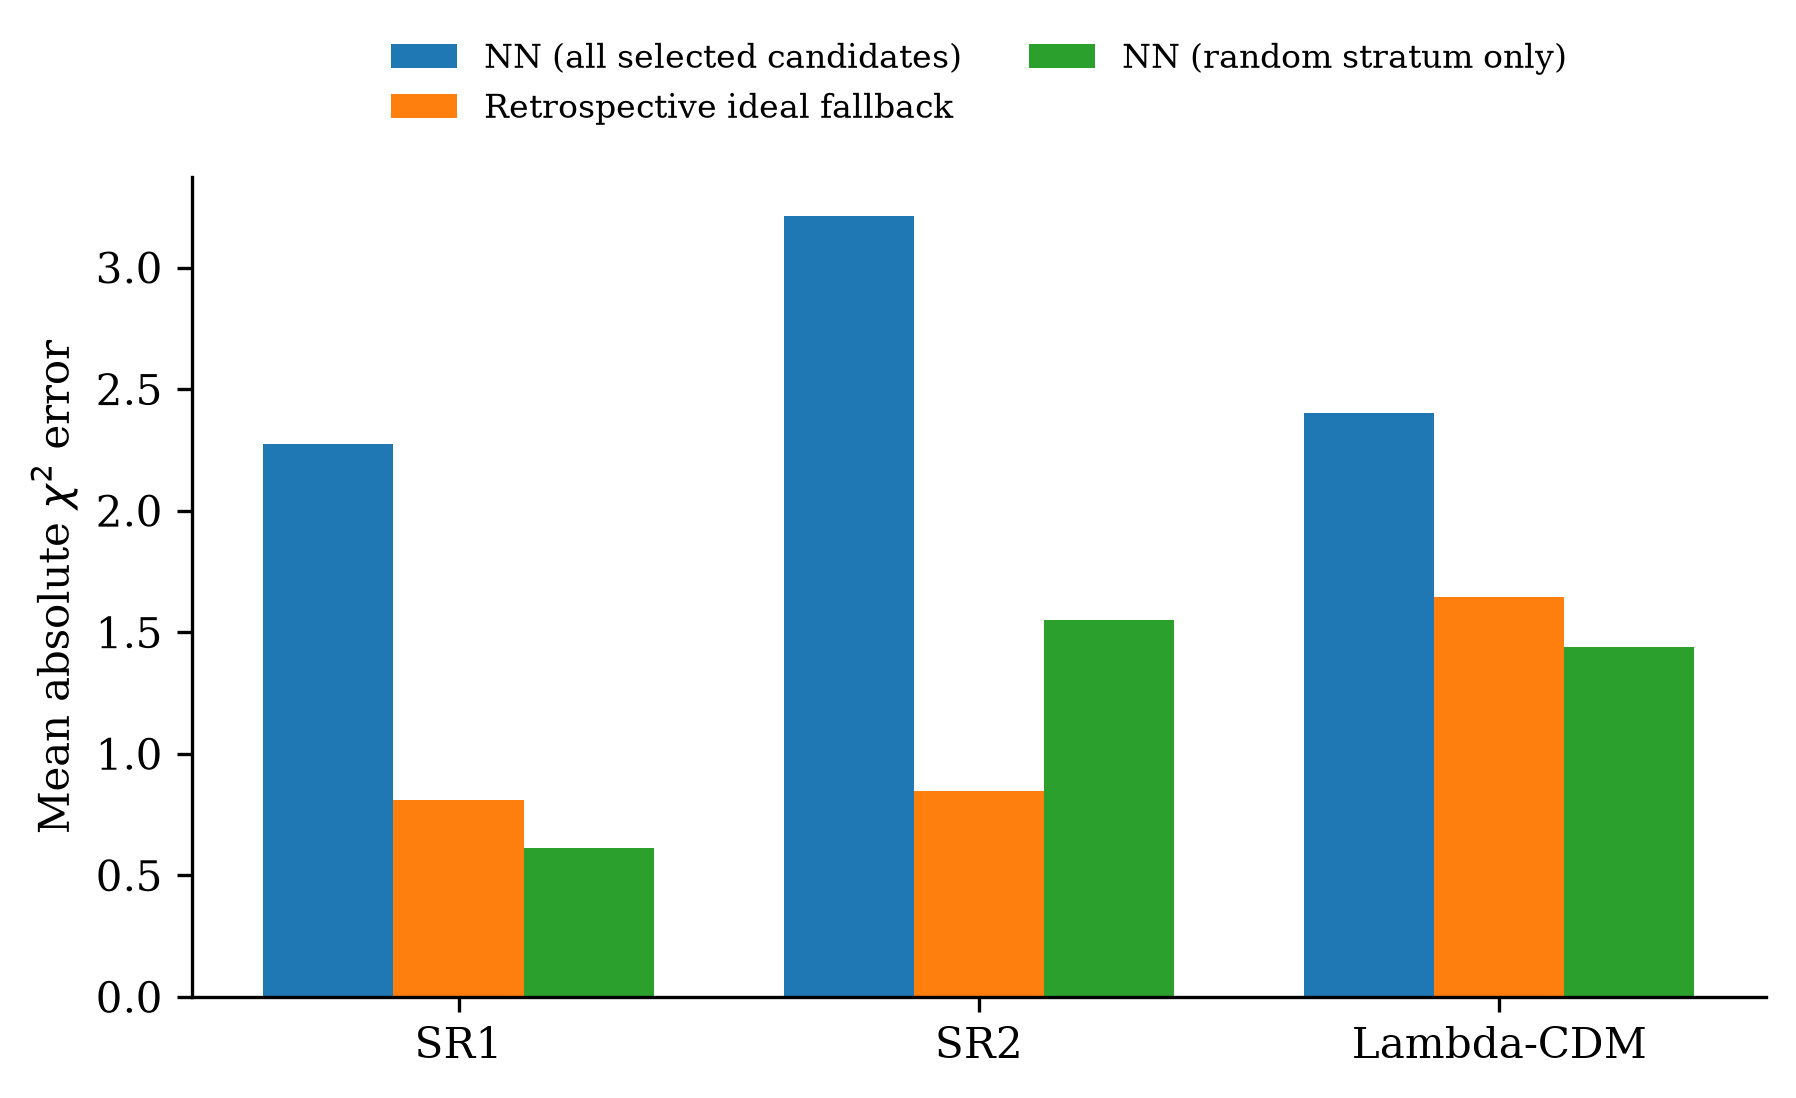
\includegraphics[width=\columnwidth]{figures/fig_error_comparison.png}
\caption{MAE on all deliberately selected candidates (blue), retrospective oracle-corrected routing (orange), and the random subset (green). The offline results do not imply measured hybrid speedup.}
\label{fig:overview}
\end{figure}

\subsection{Error and dispersion under designed validation}
External pooled MAEs are 2.274, 3.214, and 2.403 in $\chi^2$ units for SR1, SR2, and $\Lambda$CDM+$r$, respectively. The millisecond neural calls in Table~\ref{tab:perf} therefore cannot be assessed without their $\chi^2$ residuals. Mean signed residuals $\chi^2_{\mathrm{exact}}-\widehat{\chi^2}$ are positive (1.539, 3.060, and 1.454), indicating average underprediction on these selected candidates.

The pooled Spearman correlations between ensemble spread and absolute error are 0.676 (SR1), 0.488 (SR2), and 0.303 ($\Lambda$CDM+$r$). On just the 25 random candidates, they fall to 0.319, $-0.074$, and $-0.041$ (Table~\ref{tab:reliability}). Uncertainty-selected candidates also have higher MAE than random candidates: 7.104 vs. 0.611, 10.621 vs. 1.550, and 3.424 vs. 1.439, respectively. The mixed-set correlation partly reflects this deliberate selection.

\begin{table}[t]
\caption{Dispersion diagnostics and retrospective routing. $\rho_{\rm all}$ and $\rho_{\rm rnd}$: Spearman correlation on 100 mixed points and 25 random points, respectively. ``$\pm s$'' is empirical residual coverage. Routing uses offline exact-value substitution.}
\label{tab:reliability}
\centering
\footnotesize
\setlength{\tabcolsep}{3.1pt}
\begin{tabular}{@{}lrrrrr@{}}
\toprule
Model & $\rho_{\rm all}$ & $\rho_{\rm rnd}$ & $\pm s$ & Routed & Offline MAE\\
\midrule
SR1 & .676 & .319 & 15\% & 20\% & .808\\
SR2 & .488 & $-.074$ & 52\% & 21\% & .847\\
$\Lambda$CDM+$r$ & .303 & $-.041$ & 11\% & 21\% & 1.645\\
\bottomrule
\end{tabular}
\end{table}



The empirical $\pm s$ coverages are only 15\%, 52\%, and 11\%, respectively, and remain 67\%, 73\%, and 22\% within $\pm2s$. Without an independent calibration procedure, $s$ must therefore be interpreted as a ranking feature rather than a probabilistically calibrated error bound. Fig.~\ref{fig:overview} contrasts pooled and random-stratum MAE with the offline fallback experiment.

\subsection{Retrospective selective exact evaluation}
We investigate an illustrative gate that forwards roughly the highest 20\% of $s(\boldsymbol\theta)$ values to exact evaluation. The threshold is estimated out-of-fold in five partitions without consulting the held-out exact errors. For a validation record $i$, the ideal retrospective response is
\begin{equation}
\widehat{\chi^2}_{\mathrm{hyb},i}=\begin{cases}
\chi^2_{\mathrm{exact},i},&s_i>q_{0.8}^{(-i)},\\
\widehat{\chi^2}_i,&\text{otherwise},
\end{cases}
\label{eq:gate}
\end{equation}
where $q_{0.8}^{(-i)}$ denotes the threshold fitted without the held-out partition. Because exact values are already stored, this is an \emph{oracle-substitution replay}, not a runtime execution of a hybrid Cobaya sampler.

The gate routes 20--21\% of points and reduces pooled MAE to 0.808 (SR1), 0.847 (SR2), and 1.645 ($\Lambda$CDM+$r$). Every fallback belongs to the uncertainty-selected stratum; the result is selection-biased and does not establish prospective risk control.

\subsection{Retrospective posterior reweighting and tail failure}
Local predictive accuracy need not preserve Bayesian posterior
weights. For fixed priors, the surrogate-to-exact likelihood ratio is
\begin{equation}
 \frac{\widehat{\mathcal L}(\boldsymbol\theta)}{\mathcal L(\boldsymbol\theta)}
 =\exp\!\left[-\frac{\widehat{\chi^2}(\boldsymbol\theta)-
 \chi^2(\boldsymbol\theta)}{2}\right]. \label{eq:lratio}
\end{equation}
For existing PolyChord samples with normalized exact posterior
weights $w_i$, we compute the offline importance reweighting
\begin{equation}
 \widetilde w_i=\frac{w_i\exp[-(\widehat{\chi^2}_i-\chi^2_i)/2]}
 {\sum_j w_j\exp[-(\widehat{\chi^2}_j-\chi^2_j)/2]}.
 \label{eq:reweight}
\end{equation}
These are the same chain-derived coordinates used to construct the training, validation, and test partitions. Reweighting them is a stress test of likelihood substitution on a finite set, not a new posterior sample. We quantify weight concentration with Kish's $N_{\rm eff}=1/\sum_i w_i^2$, which should not be confused with autocorrelation-based MCMC ESS.

\begin{table}[t]
\caption{In-sample posterior-reweighting stress test. MAEs are for
$\chi^2$ over full chains; $N_{\rm eff}$ compares original and neural
importance weights. Tail fraction: neural weight on points where
$\widehat{\chi^2}-\chi^2<-50$.}
\label{tab:post}
\centering\footnotesize
\setlength{\tabcolsep}{3pt}
\begin{tabular}{@{}lrrrrr@{}}
\toprule
Model & $n$ & MAE & $\mathrm{MAE}_{w}$ & $N_{\rm eff}$ exact/NN & Tail \\
\midrule
SR1 & 8,474 & 130.1 & 0.685 & 2,574/18 & $>99.99\%$ \\
SR2 & 8,409 & 129.3 & 0.825 & 2,543/18 & 99.997\% \\
$\Lambda$CDM+$r$ & 9,086 & 129.8 & 1.407 & 2,724/32 & 99.997\% \\
\bottomrule
\end{tabular}
\end{table}

Despite small \emph{exact-posterior-weighted} MAEs (Table~\ref{tab:post}),
rare high-$\chi^2$ samples receive severe surrogate underestimates:
minimum $\widehat{\chi^2}-\chi^2$ reaches approximately $-1510$,
$-1496$, and $-1518$ in SR1, SR2, and $\Lambda$CDM+$r$.
For the points underestimated by more than 50, their \emph{exact}
posterior mass is $3.73\times10^{-13}$, $5.74\times10^{-13}$,
and $1.75\times10^{-11}$, respectively, yet their reweighted
mass exceeds 99.99\% in every model. The five-network dispersion
is only a few $\chi^2$ units even for several dominant outliers.
In this finite sample, reweighting gives negligible mass to the regions favored by the exact posterior and is dominated by a handful of badly underestimated points. The resulting parameter medians cannot be used as cosmological constraints. Nor can this diagnostic establish the shape of an independently sampled neural posterior.

\subsection{Targeted new-point exact verification}
For each model, we scored 12,000 perturbed chain-based proposals, then selected eight posterior-near points, eight broadly perturbed points, and eight broad points with the lowest predicted $\chi^2$. The 24 new coordinates per model were checked with the matching Cobaya--CLASS likelihood, including invalid-proposal records. These fresh evaluations test extrapolation, but are not independent posterior draws.

\begin{table}[t]
\caption{Targeted new-point checks. Valid counts and MAE in $\chi^2$
units by proposal stratum. Rejections were not assigned zero error.}
\label{tab:prospective}
\centering\footnotesize
\setlength{\tabcolsep}{3.3pt}
\begin{tabular}{@{}lrrrr@{}}
\toprule
Model & Valid & Near MAE & NN-best MAE & Wide MAE\\
\midrule
SR1 & 20/24 & 1.482 (6) & 0.636 (8) & 194.163 (6)\\
SR2 & 17/24 & 1.680 (7) & 0.658 (7) & 259.754 (3)\\
$\Lambda$CDM+$r$ & 17/24 & 2.325 (7) & 0.906 (6) & 41.425 (4)\\
\bottomrule
\end{tabular}
\end{table}

Of 72 proposals, 54 had valid exact values. Broad-group residuals reached $-490.7$, $-494.9$, and $-77.0$ for SR1, SR2, and $\Lambda$CDM+$r$, with 4, 2, and 1 errors below $-50$; valid NN-best MAEs stayed below one (Table~\ref{tab:prospective}). The deliberately selected groups, 18 invalid proposals, and small counts preclude posterior-wide inference.


\subsection{Precommitted risk gates on a new candidate set}
We compared ensemble spread $s$ with a distance score $d$: the mean Euclidean distance to five standardized reference points drawn from the 99\%-posterior-mass support. Using the 54 valid candidates from the first targeted test, we fixed 80th-percentile cutoffs for $s$, $d$, and the average of their empirical percentile ranks. Decisions and SHA-256 manifests were saved before any new CLASS evaluations.

With another seed, we generated 36 points per model (108 total) in the same three strata. CLASS returned 75 valid values; 33 points were invalid or prior-rejected. Every frozen gate flagged all 13 observed cases with $\widehat{\chi^2}-\chi^2<-50$ (Table~\ref{tab:frozen}). The spread, distance, and combined rules flagged 32, 34, and 26 proposals, respectively. Among valid, unflagged points, combined-rule MAE was 0.956--3.433. The fixed thresholds do not enforce a 20\% routing rate.

\begin{table}[t]
\caption{Held-out, precommitted combined-risk gate.
The cutoff was calibrated before exact evaluation. ``Flag'' counts
all proposals, including rejected points; MAE uses valid, unflagged
points only. All severe cases ($\widehat{\chi^2}-\chi^2<-50$) were flagged.}
\label{tab:frozen}
\centering\footnotesize
\setlength{\tabcolsep}{3.5pt}
\begin{tabular}{@{}lrrrr@{}}
\toprule
Model & Valid & Severe caught & Flagged & MAE left \\
\midrule
SR1 & 23/36 & 2/2 & 2/36 & 3.433 \\
SR2 & 28/36 & 5/5 & 12/36 & 0.956 \\
$\Lambda$CDM+$r$ & 24/36 & 6/6 & 12/36 & 2.864 \\
\bottomrule
\end{tabular}
\end{table}

Because these proposals still derive from the chains, catching 13/13 errors is a pointwise result, not a guarantee for a new sampler. A working implementation must also reject the 33 invalid points safely.

\section{Discussion and Limitations}
The timing result is unambiguous at the level measured: evaluating five neural members is far less expensive than one direct Cobaya--CLASS call. The more consequential observation is that local accuracy says little about likelihood tails. Equations~\eqref{eq:lratio} and~\eqref{eq:reweight} explain how an apparently modest surrogate prediction can reassign almost all posterior weight to points that CLASS strongly disfavors (Table~\ref{tab:post}). This is why the reweighted medians were excluded from any cosmological interpretation.

The frozen-gate test gives a more encouraging, but narrower, finding. All 13 observed severe errors were marked before their exact values became available (Table~\ref{tab:frozen}). The combined rule marked 26 of 108 proposals, compared with 32 for dispersion alone and 34 for distance alone. It did not, however, have the lowest residual MAE in every model. The same threshold need not route 20\% of later samples. Of particular concern, the proposal generator produced 33 invalid or prior-rejected candidates, which a practical implementation must check separately.

If a hybrid method calls CLASS for fraction $f$ of proposed points, its approximate mean cost is
\begin{equation}
 t_{\mathrm{hyb}}\simeq (1-f)t_{\mathrm{NN}}+ft_{\mathrm{exact}}+t_{\mathrm{gate}},\label{eq:cost}
\end{equation}
not the neural-only latency. With $f=26/108$, negligible neural and gate overhead would imply a ceiling of roughly $1/f=4.2$ on per-call acceleration, not a measured end-to-end speedup. Before any posterior-accuracy claim, we would need valid prior-aware proposals, risk calibration on representative points, a surrogate-driven sampler, and new exact calculations to check its high-probability regions.

\section{Conclusion}
For the three likelihood configurations studied here, the saved five-member ensembles reduce individual evaluation time by factors of roughly 6,800--14,600 on our benchmark node. They are useful for rapid local predictions, yet they compress portions of the high-$\chi^2$ surface severely enough to make naive importance reweighting unusable. On newly proposed points, the same extrapolation failure reappears; the best-scoring valid neural candidates are notably more accurate than widely perturbed candidates. In the separately seeded holdout, all 13 observed underpredictions beyond 50 $\chi^2$ units were identified using rules fixed before the CLASS checks. The remaining task is not another raw speed comparison, but a prospective test of whether exact fallback and prior checks preserve a posterior when the sampler itself uses the surrogate.

\section*{Acknowledgment}

OpenAI ChatGPT was used to assist with drafting and
revising text in the Abstract and Sections I--V,
preparing LaTeX material, and developing Python
scripts for computational analysis. The authors
take full responsibility for the accuracy, integrity,
and scientific content of the manuscript.

\clearpage
\begin{thebibliography}{10}
\bibitem{starobinsky1980} A.~A. Starobinsky, ``A new type of isotropic cosmological models without singularity,'' \emph{Phys. Lett. B}, vol.~91, no.~1, pp.~99--102, 1980, doi: 10.1016/0370-2693(80)90670-X.
\bibitem{blas2011} D. Blas, J. Lesgourgues, and T. Tram, ``The Cosmic Linear Anisotropy Solving System (CLASS). Part II: Approximation schemes,'' \emph{JCAP}, vol.~2011, no.~07, p.~034, 2011, doi: 10.1088/1475-7516/2011/07/034.
\bibitem{torrado2021} J. Torrado and A. Lewis, ``Cobaya: Code for Bayesian analysis of hierarchical physical models,'' \emph{JCAP}, vol.~2021, no.~05, p.~057, 2021, doi: 10.1088/1475-7516/2021/05/057.
\bibitem{handley2015} W.~J. Handley, M.~P. Hobson, and A.~N. Lasenby, ``PolyChord: Nested sampling for cosmology,'' \emph{MNRAS Lett.}, vol.~450, no.~1, pp.~L61--L65, 2015, doi: 10.1093/mnrasl/slv047.
\bibitem{planck2020} Planck Collaboration, ``Planck 2018 results. V. CMB power spectra and likelihoods,'' \emph{Astron. Astrophys.}, vol.~641, p.~A5, 2020, doi: 10.1051/0004-6361/201936386.
\bibitem{bk2021} BICEP/Keck Collaboration, ``Improved constraints on primordial gravitational waves using Planck, WMAP, and BICEP/Keck observations through the 2018 observing season,'' \emph{Phys. Rev. Lett.}, vol.~127, p.~151301, 2021, doi: 10.1103/PhysRevLett.127.151301.
\bibitem{lakshminarayanan2017} B. Lakshminarayanan, A. Pritzel, and C. Blundell, ``Simple and scalable predictive uncertainty estimation using deep ensembles,'' in \emph{Advances in Neural Information Processing Systems}, vol.~30, 2017.
\bibitem{guo2017} C. Guo, G. Pleiss, Y. Sun, and K.~Q. Weinberger, ``On calibration of modern neural networks,'' in \emph{Proc. Int. Conf. Machine Learning}, 2017, pp.~1321--1330.
\bibitem{mancini2022} A. Spurio Mancini, D. Piras, J. Alsing, B. Joachimi, and M. P. Hobson, ``CosmoPower: Emulating cosmological power spectra for accelerated Bayesian inference from next-generation surveys,'' \emph{Mon. Not. R. Astron. Soc.}, vol.~511, no.~2, pp.~1771--1788, 2022, doi: 10.1093/mnras/stac064.
\bibitem{nygaard2023} A. Nygaard, E. B. Holm, S. Hannestad, and T. Tram, ``CONNECT: A neural network based framework for emulating cosmological observables and cosmological parameter inference,'' \emph{JCAP}, vol.~2023, no.~05, p.~025, 2023, doi: 10.1088/1475-7516/2023/05/025.
\end{thebibliography}
\end{document}
